\documentclass[tikz,border=12pt]{standalone}
\usepackage{fontspec}
\setmainfont{Segoe UI}
\usepackage{amsmath,amssymb}
\usepackage{tikz}

\usetikzlibrary{calc,arrows.meta}

\begin{document}
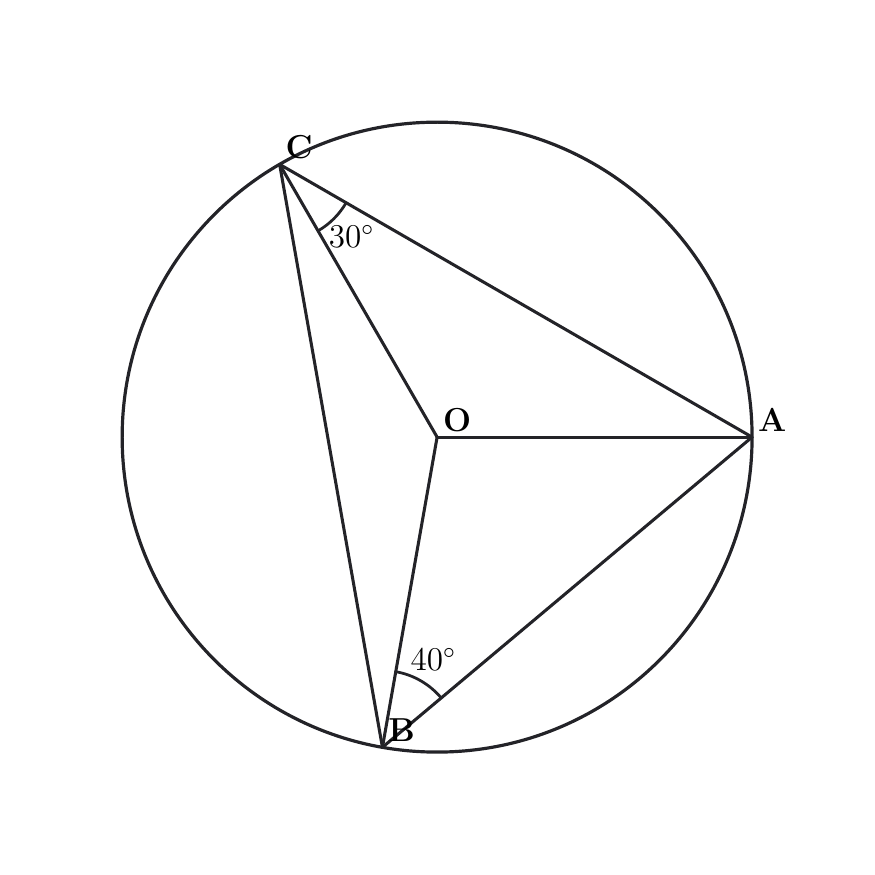
\begin{tikzpicture}[x=1.0000cm,y=1cm,line cap=round,line join=round]
\definecolor{linec0}{RGB}{35,35,40}
\definecolor{linec1}{RGB}{35,35,40}
\definecolor{linec2}{RGB}{35,35,40}
\definecolor{linec3}{RGB}{35,35,40}
\definecolor{linec4}{RGB}{35,35,40}
\definecolor{linec5}{RGB}{35,35,40}
\definecolor{edgecol}{RGB}{35,35,40}
\definecolor{hicol}{RGB}{35,35,40}
\definecolor{angcol}{RGB}{35,35,40}
\coordinate (O) at (0.0000,0.0000);
\coordinate (A) at (4.0000,0.0000);
\coordinate (B) at (-0.6946,-3.9392);
\coordinate (C) at (-2.0000,3.4641);
\draw[edgecol,line width=1.1pt] (O) -- (A);
\draw[edgecol,line width=1.1pt] (O) -- (B);
\draw[edgecol,line width=1.1pt] (O) -- (C);
\draw[edgecol,line width=1.1pt] (A) -- (B);
\draw[edgecol,line width=1.1pt] (B) -- (C);
\draw[edgecol,line width=1.1pt] (C) -- (A);
\draw[edgecol,line width=1.15pt] (O) circle [x radius=4.0000, y radius=4.0000];
\path (-5.200,-5.200) rectangle (5.200,5.200);
\draw[edgecol,line width=1.00pt] (-0.695,-3.939)++(40.00:0.975) arc[start angle=40.00, delta angle=40.00, radius=0.975];
\node[text=black,font=\large] at (-0.047,-2.818) {$40^\circ$};
\draw[edgecol,line width=1.00pt] (-2.000,3.464)++(-30.00:0.975) arc[start angle=-30.00, delta angle=-30.00, radius=0.975];
\node[text=black,font=\large] at (-1.084,2.548) {$30^\circ$};
\node[font=\bfseries\large,inner sep=2pt,anchor=south west] at (0.000,0.000) {O};
\node[font=\bfseries\large,inner sep=2pt,anchor=south west] at (4.000,0.000) {A};
\node[font=\bfseries\large,inner sep=2pt,anchor=south west] at (-0.695,-3.939) {B};
\node[font=\bfseries\large,inner sep=2pt,anchor=south west] at (-2.000,3.464) {C};
\end{tikzpicture}
\end{document}
